\subsection{Existing Products and Projects}
% how have other projects and products used similar strategies to FORWARD?

\noindent There have been numerous efforts made by researchers to develop smart walkers using the available technologies. Perhaps the seminal work in this growing field of research and development is \cite{PAMM}. This group was the first to propose a smart walker project with localization, mobility control, and object avoidance. In the following sections we seek to analyze these technologies and methods in a way that identifies which of such will be most desired for our specific system, taking into consideration many factors, some of which being: cost, attainability, integration complexity, and performance.

%% Toby research here
\subsubsection{Current Walker Sensing Applications}
\noindent In the smart walker prototype created in \cite{Mostofa}, nine HC-SR04 ultrasonic sensors are arrayed along the front of the walker. Seven face forward, while the remaining two point perpendicularly to the walker motion and opposite to each other. This setup provides a continuous reading of the walker's forward hemisphere with a detection range of 200cm. Our team asks the question, can obstacle detection and notification be achieved with a more discrete array of sensors stowed onto the walker frame? What is the operational FOV for ultrasonic sensors? Can the amount be reduced? How will the introduction of LiDAR and camera technology affect the ultrasonic approach?\\

\begin{figure}[h]
	\centering
	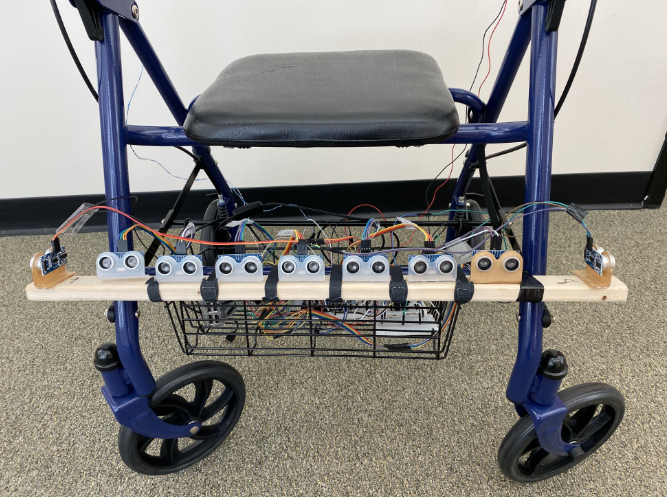
\includegraphics[width=0.5\textwidth]{./Images/mostafa9.png}
	\caption{\label{fig:mostafa9}"Rollator" with nine HC-SR04 sensors \cite{Mostofa}}
\end{figure}

\noindent Robotics are a popular use of LiDAR, often able to achieve feats such as autonomous delivery. However, many researchers have also introduced laser sensing methods and other waves near infrared in order to provide ranging data to mobile systems, which in our case is the walker. A senior design group at Michigan State University expanded on this \cite{mstate}.\\

\noindent In \cite{FallDetect}, the group implements one of FORWARD's stretch features with an unorthodox yet clever utilization of LiDAR and sensor fusion. In order to equip the walker with fall detection, both ultrasonic and laser sensors are installed near the footstep bay of the walker. They also add force sensors in the handlebars. The feedback provided by the sensing system is whether the user is walking uprightly. If the user began to fall, the laser sensors would reflect their feet moving out of view, and likely the force sensors would experience more pressure as the user reacted to a slip. \\

\noindent This walker does not employ GPS. We are not looking to track the location continuously. This technology has more of a place within the application of health monitoring and emergency alerts.\\

\subsubsection{Current Computer Vision Object Detection Applications}
\noindent There have been multiple attempts to exploit the current state of machine learning and AI to bring guidance to the visually impaired. Many of the existing projects implement the YOLOv5 model to develop their object detection algorithms.\\

%https://www.mdpi.com/2227-7080/11/6/168
%https://www.sciencedirect.com/science/article/pii/S2090447923002769

%% Matthew Research Here

%% Morgan Research Here
\subsubsection{Motor and Steering Applications} 

